% TEMPLATE for Usenix papers, specifically to meet requirements of
%  USENIX '05
% originally a template for producing IEEE-format articles using LaTeX.
%   written by Matthew Ward, CS Department, Worcester Polytechnic Institute.
% adapted by David Beazley for his excellent SWIG paper in Proceedings,
%   Tcl 96
% turned into a smartass generic template by De Clarke, with thanks to
%   both the above pioneers
% use at your own risk.  Complaints to /dev/null.
% make it two column with no page numbering, default is 10 point

% Munged by Fred Douglis <douglis@research.att.com> 10/97 to separate
% the .sty file from the LaTeX source template, so that people can
% more easily include the .sty file into an existing document.  Also
% changed to more closely follow the style guidelines as represented
% by the Word sample file. 

% Note that since 2010, USENIX does not require endnotes. If you want
% foot of page notes, don't include the endnotes package in the 
% usepackage command, below.

% This version uses the latex2e styles, not the very ancient 2.09 stuff.
\documentclass[letterpaper,twocolumn,10pt]{article}
\usepackage{usenix,epsfig,endnotes}
\usepackage[backgroundcolor=yellow]{todonotes}
\usepackage{cite}
\usepackage{subfig}
\usepackage{xspace}
\usepackage{graphicx}
\usepackage{hyperref}
\usepackage{epstopdf}
\usepackage{tabularx}
\usepackage{array}
%\usepackage{graphicx}

\usepackage{amsmath}
%\usepackage{subcaption}
\usepackage{xcolor}

\usepackage{adjustbox}
\usepackage{multirow}

\usepackage{todonotes}
\newcommand{\MM}{Artifice}
\newcommand{\mfs}{Artifice\xspace}
%\usepackage[hyphens]{url}
%\usepackage[breaklinks]{hyperref}
\newcommand{\etal}{\emph{et~al.}\xspace}
% Name definitions
%\newcommand{\SYS}{artifice\xspace}
%\newcommand{\SYSB}{OSP\xspace}
\newcommand{\eg}{\emph{e.g.}\xspace}

\pagenumbering{gobble}

\begin{document}

%don't want date printed
\date{}

%make title bold and 14 pt font (Latex default is non-bold, 16 pt)
\title{\Large \bf Approachable Cryptography}

%for single author (just remove % characters)
\author{
{\rm Austen Barker}
\and
{\rm Staunton Sample}}
%\and
%Univ.~of California, Santa Cruz
%}  % end author
% copy the following lines to add more authors
% \and
% {\rm Name}\\
%Name Institution

\maketitle

% Use the following at camera-ready time to suppress page numbers.
% Comment it out when you first submit the paper for review.
%\thispagestyle{empty}

\renewcommand{\thefootnote}{\fnsymbol{footnote}}
\subsection*{Abstract}
Significant issues arise when implementing modern cryptographic algorithms in generic programming languages. Cryptography has a storied yet flourishing research community. Yet this is mostly based in the notation of Mathematics. This create issues when production environments must utilize algorithms with high use cases. A Domain Specific Language(DSL) can possibly be used to bridge this divide. Our project proposes an exploration of the research behind, and implementation of, Domain Specific Programming languages purposed for Encryption.  We examine four modern generic programming languages by implementing the Rivest Cipher 4(RC4), and benchmarking the results. We also implement RC4 in Cryptol, an encryption DSL, for comparison.

\section{Introduction}
While the theoretical creation and proving of cryptographic algorithms has a strong and rigorous foundation, the implementation of the same algorithms in computer programs faces significant hurdles due to challenges presented by generic programming languages. Specifically, widely used languages such as C, Java, LISP, Python pose language specific problems regarding information leakage and lack of performance when implementing modern cryptography \cite{Lewis}. Even more troubling can be the difficulty in simply understanding the written algorithm or writing the algorithm due to a lack of tools \cite{Agosta}. In this project, we discuss previously proposed Encryption Domain Specific Languages and explore the need for an alternative encryption based Domain Specific Language(DSL).  We also study the challenges faced by modern languages by implementing and benchmarking a modern cryptographic algorithm, RC4, in C, Java, Python, and LISP. Furthermore, we also implement RC4 in Cryptol, a modern and maintained Encryption DSL to provide a counterpoint to the generic language implementations with the hypothesis that Cryptol, or another Encryption DSL, can be as performant as the generic languages while improving readability and and providing provable correctness.


\section{Background}
There exists minimal research into the area of Domain Specific Languages for Encryption algorithm development and verification. With that in mind, we will discuss what does currently exist in regards to previous research on the topic.

\subsection{Domain Specific Languages}
 A Domain Specific Language is a programming language specifically designed to facilitate purpose driven coding. DSL's can be divided into markup, modeling, and programming. Our exploration of previous work will only discuss Programming Domain Specific Languages. 

According to Mernik \cite{Mernik}, a Domain Specific Language should offer the following advantages over a generic language: DSL's should have notation based on, or similar to, an existing and established syntax, inclusion of abstraction of the intended domain, and the ability for automatic transformation. Specific to Encryption DSL's, the language design should include the notation elements that support Number theory and Advanced Algebraic concepts. Furthermore, the design would need to incorporate the analysis, verification, parallelization, and optimization necessary to support implementation for modern hardware and software systems. Finally, any DSL design for encryption must allow for specific crytptographic data structures that facilitate operations such as multi precision numbers, univariate polynomials, and compositions of polynomials \cite{Agosta}.

In keeping with these specifications, Agosta and Pelosi \cite{Agosta} attempt to create an  Encryption DSL library based on Python. The library supports both unlimited precision and fixed precision data types by allowing each data type to specified by a size extension. Furthermore, in their library it is possible to specify a user-defined data type with a traditional array construct, or for encryption specific data types, modular arithmetic and polynomial data types can called with built in commands. The framework further supports scalar and vector operators, and maintains python style function declaration to better cope with lower level specifications.

Nielsen and Schwartzbach \cite{Nielsen} describe a programming language for secure multiparty communication. While this approach does not focus specifically on a language for the development and testing  of encryption algorithms, it does attempt to bridge the gap between high-level requirements and low level development. This focus provides a framework for development with a distinction between client and server with built-in, provably secure tunneling.  While their proposal is an imperative style DSL, they do not formally address how side effects created by primitive operations affect provable security.

A homomorphic encrytption platform is proposed by Bain et al. \cite{Bain}. This platform would support secret sharing execution while discourage leaks by server collusion. The DSL is built on Haskell and C++ and avoids any unusual language restrictions by relying on the Haskell type system. More specifically, the Haskell constructs employed are monads and type classes. Though, it is not clear from the paper whether or not there is an actual formal verification system that is incorporated.  

With cPLC, Bangerter et al. \cite{Bangerter} propose a compiler and implementation language for two-party cryptographic protocols. The paper focuses mostly on compiler design and implementation leaving only a small discussion regarding the inclusion of the input language. Furthermore, the input language uses branching and loops which are known to cause information leakage. 


\subsection{Cryptol}
Cryptol is a high specification Encryption Domain Specific Language first developed by the National Security Agency and currently maintained by Galois Inc. Cryptol was originally developed for Field Programmable Gate Array based encryption specific hardware \cite{Lewis}. Built on top of Haskell, Cryptol offers the ability to write, secure implementations of algorithms and be immediately verified for correctness. This sets Cryptol apart as implementations are hardware and platform independent for provable correctness. Cryptol uses uniform sequence expression \cite{Lewis}. Bits are handled as an array of booleans, where one is equal to True. Numbers are represented with bit vectors and modulus arithmetic. Polynomials are supported with through traditional mathematical notation. Finally, control flow and loops are avoided as they provide opportunity for information leakage. 

\subsection{Implementing Cryptographic Algorithms}
There are many considerations that must be taken into account while implementing cryptographic algorthims and cipher or more broadly anything related to the security of 
a computing system\cite{CryptoCoding}. One could easily produce multiple papers giving just an overview of the problems programmers face. We limit ourselves to a relatively brief overview.

First is the issue of comparison methods. If a programmer uses a comparison method for two secret pieces of information which possesses a runtime analogous to the length 
of the secret data the program is difficult to a timing attack. In which an adversary derives the length of a secret from the amount of time taken to process the secret. 
Leaking the length of a secret piece of information drastically reduces the search space for a brute force attack against a cipher. A solution for this is to use a 
constant time comparison method which is not common used in many languages. A similar issue exists when branches (loops or recursion) are controlled by secret data. The 
number of iterations can betray the length of the secret.

Compiler or interpreter optimizations must be conciously avoided as they can introduce unintended behavior into the executing program. For instance some compilers will 
optimize out \texttt{memset} operations used to set a piece of memory that once held a secret to all zeros.

Data type selection is crucial in cryptographic applications. All binary data must be represented by unsigned bytes. Not using unsigned data types or some workaround allows 
for buffer overflow and underflow errors to compromise the operational correctness of an implementation. It is also not advisable to use different data types for secret or 
non-secret information as different types will let an adversary identify pieces of data as secret or non-secret.

Lastly many languages either have built in calls to generate random numbers or provide libraries to do so. These random number generators are often not suitable for use 
in cryptographic applications as they do not achieve the required level of entropy. A programmer must be concious of their source of random number and select those that are 
cryptographically secure such as the Linux/Unix kernel's \texttt{/dev/random}.

\subsection{RC4}

Rivest Cipher 4 (RC4), also known as ARC4, is a relatively common and simple stream cipher that we have 
used for evaluating different languages in terms of their ability to securely and reliably implement 
cryptographic algorithms. In a stream cipher a stream of pseudorandom bits are generated and then combined 
with the plaintext via an operation such as a bitwise exclusive-or (XOR). The cipher consists of two main 
components, a key scheduling algorithm (KSA) and a pseudo-random generator algorithm (PRGA). The key scheduling algorithm 
takes in a supplied key to generate a permutation of all $256$ possible bytes. This is used a seed for the 
PRGA which iterates over the permutation of bytes generating a pseudo-random key stream equal in length to 
the plaintext. This key stream is then combined with the plaintext using a bitwise XOR. The same operation is 
then repeated in order to retrieve the plaintext.


\section{Implementation}
In order to evaluate the need for a domain specific programming language we implemented a basic stream cipher, RC4, 
in a variety of different programming languages. Although it is no longer commonly used or secure, RC4 encompasses 
the basic bitwise operations necessary for implementing cryptographic algorithms. We focus on the base functionality 
of each language and ignore most libraries and API functions beyond what is absolutely necessary. In the case of C we 
assume that the same behavior observed is also true for C++.

\subsection{C}
Commonly used for implementing cryptographic algorithms for kernel development, systems libraries, and embedded applications 
where there is no hardware implementation. C provides maximum freedom out of our implementations as the programmer has access 
to the actual memory locations where data is stored. In the hands of a competent and attentive programmer C allows for maximum 
performance and an assurance that certain memory operations have taken place. Such as zeroing memory with \texttt{memset()} used to store a key after 
it has been freed. Bitwise operations and substitution is relatively easy in C even though there is no access to individual bits. The representation of 
Strings as an array of characters also makes it easy to convert them into arrays of bytes. Lastly, the presence of a multitude of different unsigned 
data types and type checking at compile time helps to protect the programmer from easy mistakes. Most errors, such as type issues, in a program are 
also caught at compile time therefore avoiding costly mistakes from appearing in a production environment.

The same flexibility that manual memory management that C provides is also its greatest weakness. The danger of a buffer overflow is significant with 
applications written in C. Commonly used operations such as \texttt{strcpy()}, \texttt{gets()}, and \texttt{strcmp()} do not check the length of 
their inputs therefore leaving any program using them vulnerable to carefully selected inputs which can leak information. For instance calling any 
string comparison method, like \texttt{strcmp()}, which compares two strings character by character will leak the length of said string. A programmer must also be 
careful when determining the size of a piece of data in memory. If using a structure for managing data padding can be inserted between variables and when the 
function \texttt{sizeof()} is called on a pointer it returns the length of a memory address, not the data at that memory address. Compilers and the standard 
library also pose issues. The standard library is used for many basic operations in C but sadly many parts of this library such as the random number generator 
are not cryptographically secure. Most C compilers offer some form of optimization that can introduce inintended or undefined behavior into the resulting 
program. For instance undefined behavior is especially common when using the second and third optimization settings with the Gnu C Compiler.

\subsection{Lisp}
Among the many dialects of Lisp available we used Common Lisp, primarily due to its popularity as the name would imply. Lisp allows us to represent our plaintext, 
ciphertext, and key as lists of bytes. Which allows for relatively simple bitwise operations even though as with C we have no access to individual bits. The functional
paradigm also lends itself well to how cryptographic algorithms are constructed. With multiple operations occuring one after the other on a stream of data. The primary 
advantage of Lisp is that it is a garbage collected language. Unlike C this means that the language is memory safe. While enforcement of limits on allocated 
regions of memory removes the possibility for things like buffer overflow and misjudging the size of a region in memory it also hides what machine code is actually 
being executed.

\subsection{Python}
While celebrated for its simplicity, accessibility and similarity to pseudocode often used to express cryptographic algorithms in specifications. Our KSA and PRGA 
in Python are virtually identical to the pseudocode used as a basis for all our implementations. Python is not very well suited to the task of implementing 
cryptographic algorithms. Primarily due to its weak type system that does not enforce anything before running a program. In addition to this major flaw occassionally type 
errors never appear as the Python interpreter may perform implicit type conversions at runtime.

\subsection{Java}
As one of the most commonly used programming languages and a prime example of an object oriented paradigm, Java is an obvious choice for our lineup of programming languages.
Syntactically Java is similar to C and in some cases identical for many of the operations that are used in implementing RC4. The biggest difference being that Java manages 
memory for the programmer and that it lacks a data type for an unsigned byte. This first point is more of an advantage than a drawback as manual memory management is the 
source of most of the weaknesses in C. Although it does open the door for uncertaintly about what is actually being executed by the Java Virtual Machine and whether or not 
its memory is securely being freed. The lack of an unsigned byte type in Java means that while one can represent a stream of bytes as an array, one must either use multiple 
API functions such as a \texttt{BitSet} or juggle type casting and bit masking each time an operation on an individual byte is desired. There is also the fact that 
strings are represented as Java objects instead of as a primitive data type so a user is not entirely sure what could be leaked when converting a string into an array of 
bytes.

\subsection{Cryptol}
The strong typing explicitly declared by the programmer preceding each function that was inherited from Haskell puts Cryptol well ahead of its competition in terms of 
type systems.

\section{Evaluation}
Here we compare our implementations of RC4 in terms of performance, lines of code, and a qualitative analysis. For performance we measure latency and throughput for 
each implementation with the exception of Cryptol as we have not yet found an effective way to benchmark its performance.

\subsection{Performance}

We evaluated the performance of our implementations for both latency and throughput. In order to measure this we encrypted Mark Antony's 
monologue from Act $3$ Scene $2$ of Shakespeare's play \emph{Julius Caesar} using a relatively short 12 character key. We used Python version 2.7, OpenJDK 8, GNU Clisp 2.49, SBCL 1.3.1, and GCC 5.4. Due to the large variability between the behavior of Common Lisp interpreters we evaluated 
two of the most common GNU Clisp and SBCL.

\begin{figure}
\centerline{ 
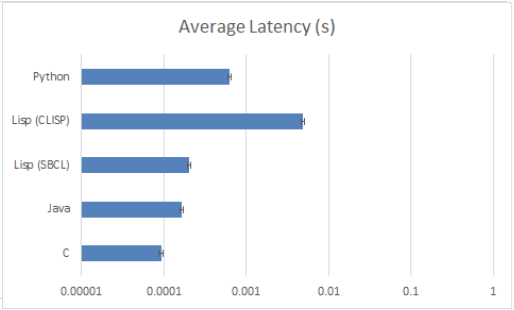
\includegraphics[width = 0.5\textwidth]{latency.PNG}}
\caption{Latency for encrypting or decrypting bytes.}
\label{fig:lan}
\end{figure}

We can see here that the fastest language by far is C with just under 100 milliseconds. Closely following is Java and the SBCL Lisp result. The Python and GNU Clisp results are the slowest. Especially the GNU lisp with a latency almost approaching one hundreth of a second.

\begin{figure}
\centerline{ 
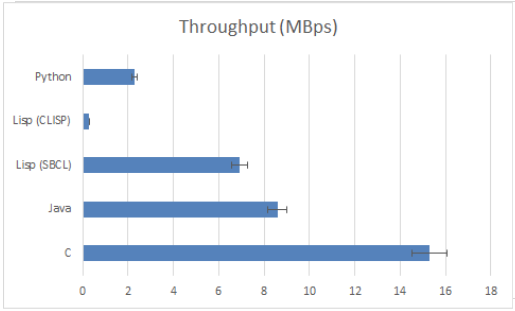
\includegraphics[width = 0.5\textwidth]{throughput.PNG}}
\caption{Latency for encrypting or decrypting bytes.}
\label{fig:lan}
\end{figure}

Similar trends are shown in the throughput. With C being the leader, followed in the same order by Java, SBCL, Python, and GNU Clisp.


\subsection{Qualitative Analysis}

No language, even Cryptol, adequately protects against timing attacks as each will allow a programmer to utilize the length of a secret 
to define the number of iterations in a recursive statement or a loop. This is a difficult issue as it would require the programmer to 
either classify a piece of data as a secret, perhaps similarly to how a variable can be \texttt{const} or \texttt{static} in C.


\section{Conclusion}



%\section{Acknowledgments}
%Thanks people

{\footnotesize \bibliographystyle{acm}
\bibliography{203}

%\theendnotes

\end{document}
